\documentclass[letterpaper, 10 pt, conference]{../ieeeconf} 
\IEEEoverridecommandlockouts
\overrideIEEEmargins
\pdfoptionpdfminorversion=4

\usepackage{amsmath}
\usepackage{mathtools}
\usepackage{textcomp}
\usepackage{graphicx}
\usepackage[font=footnotesize]{subcaption}
\usepackage[font=footnotesize]{caption}
\usepackage{hyperref}
\usepackage{amssymb}
\usepackage{booktabs}
\usepackage[normalem]{ulem}
\usepackage{verbatim}
\usepackage[export]{adjustbox}
\usepackage{amsmath}
\usepackage{url}
\usepackage{siunitx}
\usepackage[utf8]{inputenc}
\usepackage[TS1,T1]{fontenc}
\usepackage{array, booktabs}
\usepackage{caption}
\usepackage[cal=cm]{mathalfa}
\usepackage{algorithm}
\usepackage[noend]{algpseudocode}

% Labels in IEEE format
\newcommand{\eref}[1]{(\ref{#1})} % Equation
\newcommand{\sref}[1]{Sec.~\ref{#1}} % Section
\newcommand{\figref}[1]{Fig.~\ref{#1}} % Figure
\newcommand{\tref}[1]{Table~\ref{#1}} % Table
\newcommand{\aref}[1]{Algorithm~\ref{#1}} % Algorithm
\newcommand{\lref}[1]{Line~\ref{#1}} % Line
\renewcommand*\rmdefault{ppl}
\setlength{\textfloatsep}{5pt}

\usepackage{ifthen}
\usepackage[usenames,dvipsnames,table]{xcolor}
\newboolean{include-notes}
\setboolean{include-notes}{true} 
% http://en.wikibooks.org/wiki/LaTeX/Colors
\newcommand{\rhnote}[1]{\ifthenelse{\boolean{include-notes}}%
 {\textcolor{red}{\textbf{RH: #1}}}{}}
\newcommand{\sanote}[1]{\ifthenelse{\boolean{include-notes}}%
 {\textcolor{green}{\textbf{SAN: #1}}}{}}

\begin{document}

% paper title
\title{6.857 Final Project: Milestone 6}
\author{Sebastiani Aguirre Navarro and Rachel Holladay}
\maketitle

\begin{abstract}
The goal of this project was to use modified depth images to perform binary classification whether a grasp would succeed, as measured by a grasp stability metric. 
We utilize the Dex Net 2.0 data base of grasp, images and stability labels~\cite{mahler2017dex}.
We begin by training variants of the data set with the Dex Net learning architecture before exploring a variety of different network structures. 
\rhnote{overall results}
\end{abstract}

% !TEX root = main.tex

\section{Introduction}
\label{sec:intro}

The ability to grasp objects lies at the heart of robotic manipulation and therefore is fundamental to enabling robots to have complex physical interactions with their environment. 
Grasping a variety of unknown objects is challenging due to sensor and actuator uncertainty and uncertainty with respect to a new object's shape, mass distribution, texture properties, etc. 
Recently, deep neural networks have been used, with significant success, to address these challenges and enable robotic grasping. 

Within the context of this paper, we will make three assumptions. 
First, we will be grasping objects from a flat, clutter-free surface, such as an uncrowded table top. 
Second, we assume we have a method of generating \textit{grasp candidates}. 
Last, the robot has either an on-board camera or the environment the robot is operating in has a camera. 
Given an image of the scene captured by the camera, our goal is to evaluate which of these candidate grasps are likely to succeed. 
This creates a binary classification task, where the labels are grasp success and grasp failure. 

During execution, we can imagine that our robot with sample several grasps, execute a grasp that has been predicted to be successful via our classification method.  

For our data set we will use the Dexerity Network (DexNet) 2.0 data set, presented in~\cite{mahler2017dex}. 
The data set has 6.7 million grasps definitions, images and analytical grasp metrics, that we further detailed in \sref{sec:data_set}. 
The authors of the data set trained a Grasp Quality Convolutional Neural Network (GQ-CNN), which achieved 85.7\% accuracy on their classification task.

Using their network, on both our sampled data and their provided data, we were unable to achieve an accuracy rate higher then the percentage of the largest class. We discuss several possible reasons. We then explore several other architectures, with varying hyper parameters and normalization methods. 

\textbf{We make the following contributions}:
\begin{enumerate}
    \item \rhnote{fill in}
		\item \rhnote{fill in}
\end{enumerate}

We first review related work (\sref{sec:related_work}) and further detail the data set (\sref{sec:data_set}). 
Given our data set, we formally define our problem statement (\sref{sec:problem}) and then explore various data sets using the pre-trained GQ-CNN (\sref{sec:balance}). 
We explore other architectures (\sref{sec:archs}) and conclude with a brief discussion (\sref{sec:discussion}). 

\begin{figure}[t!]
    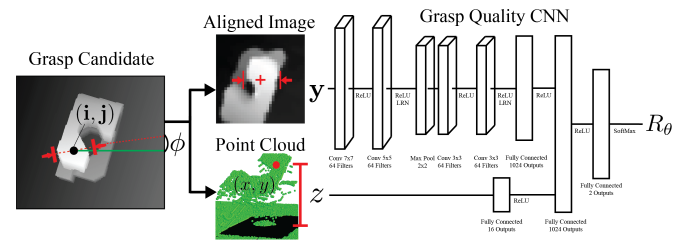
\includegraphics[width=0.99\columnwidth]{figs/dexnet.PNG}
\caption{This is a visualization the GQ-CNN (Grasp Quality Convolutional Neural Network) from \cite{mahler2017dex}. The network takes as input a depth image of the grasp and the distance of gripper to the object and output, after several layers, a prediction of grasp success.} \label{fig:dexnet_network}
\end{figure}

\begin{comment}

To accomplish the same task, we will be experimenting with new architectures, input formats, other modifications described in~\sref{sec:questions}.
Most of the recent machine learning papers in robotics present a problem, dataset and, usually, an optimized convolutional neural network with some architecture and input format. 
Our goal is to explore the process of finding that CNN and exploring the factors that effect performance. 
While our results will only be verified according to this data set, and therefore cannot be generalized to all CNNs, we hope to gain intution, understanding, and, hopefully, a higher accuracy. 
Having explored various components, we will optimize our final, best architecture. 
\end{comment}

% !TEX root = main.tex

\section{Related Work}
\label{sec:related_work}

While we primarily build off of the Dex Net 2.0 paper~\cite{mahler2017dex}, there is a wide range of literature investigating learning how to grasp objects. 
The overwhelming majority of the recent work has focused on using CNNs, although there are a few papers that use SVMs, kernel-density estimation and constrained optimization-based techniques~\cite{jiang2011efficient,kopicki2016one,el2012bridging}. 

Ten Pas et al~\cite{pas2017grasp} developed a grasp detection algorithm similar to the Dex Net paper by generating grasp hypotheses and training a 4-layer CNN to perform binary classification on whether the grasp is viable. 
They use a different grasp representation and rely on the BigBird data set~\cite{singh2014bigbird}. 
Rather then classifying a grasp, Johns et al uses a CNN to learn a grasp function, which provides a score for each grasp~\cite{johns2016deep}. 
At execution time, then can compare the scores of several grasps and select the best grasp.

The above works focus on using a parallel jaw gripper, a two finger hand where the fingers are parallel to each other and usually move together. 
While this is a relatively simple hand, it is ubiquitous in industry and research and still allows for complex manipulation tasks~\cite{mason2011generality}. 
However, people have worked to expand this grasp prediction to more complex, multi-fingered hands using various CNN architectures~\cite{luplanning,varley2015generating,zhou20176dof}. 

Within the grasp learning community, and in fact, within the robotics learning community, there is a pull between real data collected through a robotic platform and data generated from a physics simulator. 
While data collected on a robot better captures reality (since physics simulators are far from perfect), data collection is difficult and time-consuming. 
Pinto et al collected, at the time, a record amount of data at 50k data points of grasps collected across 700 robot hours~\cite{pinto2016supersizing}.
Levine et al later collected 800,000 grasp attempts over a two month period, using between six and fourteen robot arms at once~\cite{levine2016learning}. 
While these approaches allowed them to train a CNN without over fitting or using simulation data, such data collection is not always practical and require a huge amount of engineering effort. 
Bousmalis showed how to augment a smaller amount of real data with simulation to improve accuracy, thus attempting to combine the merits of both~\cite{bousmalis2017using}. 

While most of this work focuses on using color (RGB) or depth (RGBD) images~\cite{lenz2015deep}, there is growing interest in using tactile feedback, inspired by how humans feel as they grasp. 
Calandra et al combines vision and touch sensing to build a visuo-tactile CNN that predicts grasp outcomes from a combination of the modalities~\cite{calandra2017feeling}. 
This can go one step further in using tactile feedback to learn how to readjust while grasping~\cite{chebotar2016self}. 

Dex Net 2.0 is the second of three pieces of research. 
Dex Net 1.0 solves the same grasping problem, but uses a multi-armed bandit model to correlate the rewards of a proposed grasp with previously seen grasps~\cite{mahler2016dex}.
The similarity metric between grasps is learned from a Multi-View CNN. 
Dex Net 3.0 uses a CNN to learn suction points, leveraging recent interest in using suction for pick and place motions~\cite{mahler2017suction}. 

\begin{comment}
BigBird is "a high-quality, large-scale dataset of 3D object instances, with accurate calibration information for every image. We anticipate that “solving” this dataset will effectively remove many perception-related problems for mobile, sensing-based robots."~\cite{singh2014bigbird} 

Grasp detection algorithm for cluttered environments. Generate grasp hypothesis, develop description. Sample a bunch of these and then do binary classification task using a 4-layer CNN. Use big bird~\cite{pas2017grasp}

In this paper, we take the leap of increasing the available training data to 40 times more than prior work, leading to a dataset size of 50K data points collected over 700 hours of robot grasping attempts. This allows us to train a Convolutional Neural Network (CNN) for the task of predicting grasp locations without severe overfitting. In our formulation, we recast the regression problem to an 18-way binary classification over image patches (model grasp-able from different angles)~\cite{pinto2016supersizing}

Detect grasps from RGBD image. Two layer network, early deep learning grasping paper, deals with rgbd instead of just rgb image~\cite{lenz2015deep}. 

grasp proposals from images (not deep learning). focused on novel objects. more descriptive grasp representation, use SVMs \cite{jiang2011efficient}

estimate grasp robustness from local contact patch (use deep learning and random forest)~\cite{seita2016large}

we use dex net 2.0 which builds off of dex net 1.0. This paper presents the Dexterity Network (DexNet) 1.0, a dataset of 3D object models and a sampling-based planning algorithm to explore how Cloud Robotics can be used for robust grasp planning. The algorithm uses a MultiArmed Bandit model with correlated rewards to leverage prior grasps and 3D object models. Dex-Net 1.0 uses Multi-View Convolutional Neural Networks (MV-CNNs), a new deep learning method for 3D object classification, to provide a similarity metric between objects~\cite{mahler2016dex}

present a grasp stability predictor that uses spatio-temporal tactile features collected from the early-object-lifting phase to predict the grasp outcome with a high accuracy. then used to learn grasp readjustments. \cite{chebotar2016self}

action condition video prediction over pixel movement to learn physical interactions, use on a dataset of 59,000 robot interactions involving pushing motions,\cite{finn2016unsupervised}

Deducing whether a particular grasp will be successful from indirect measurements, such as vision, is therefore quite challenging, and direct sensing of contacts through touch sensing provides an appealing avenue toward more successful and consistent robotic grasping. However, in order to fully evaluate the value of touch sensing for grasp outcome prediction, we must understand how touch sensing can influence outcome prediction accuracy when combined with other modalities. Build  visuo-tactile deep neural network models to directly predict grasp outcomes from either modality individually, and from both modalities together. \cite{calandra2017feeling}

learning-based approach to hand-eye coordination for robotic grasping from monocular images. To learn hand-eye coordination for grasping, we trained a large convolutional neural network to predict the probability that taskspace motion of the gripper will result in successful grasps, using only monocular camera images independent of camera calibration or the current robot pose~\cite{levine2016learning}

Dex Net 3.0 uses suction instead, with CNN\cite{mahler2017suction}. 

Hard to collect real robot data. Want to use simulation but simulation doesnt model world precisely. We study how randomized simulated environments and domain adaptation methods can be extended to train a grasping system to grasp novel objects from raw monocular RGB images. (improve accuracy with good simulation and first to use monocular rgb)~\cite{bousmalis2017using}


This paper presents a new method for paralleljaw grasping of isolated objects from depth images, under large gripper pose uncertainty. Whilst most approaches aim to predict the single best grasp pose from an image, our method first predicts a score for every possible grasp pose, which we denote the grasp function. To learn this function, we train a Convolutional Neural Network which takes as input a single depth image of an object, and outputs a score for each grasp pose across the image. Training data for this is generated by use of physics simulation and depth image simulation with 3D object meshes. rhnote{Use same structure as alexnet}~\cite{johns2016deep}

novel approach to multi-fingered grasp planning leveraging learned deep neural network models. We train a convolutional neural network to predict grasp success as a function of both visual information of an object and grasp configuration. We can then formulate grasp planning as inferring the grasp configuration which maximizes the probability of grasp success~\cite{luplanning}

This paper presents a method for one-shot learning of dexterous grasps and grasp generation for novel objects. A model of each grasp type is learned from a single kinesthetic demonstration and several types are taught. These models are used to select and generate grasps for unfamiliar objects. Both the learning and generation stages use an incomplete point cloud from a depth camera. model uses kernel-density estimation. ~\cite{kopicki2016one}

deep learning architecture
for detecting the palm and fingertip positions of stable grasps
directly from partial object views. multi-finger. model is learning grasp quality metrics. Deep Model with local contrast normalization (LCN), 5 convolutional layers, and 3 fully connected layers. experiment with different parameters~\cite{varley2015generating}

s paper considers learning grasps in the full 6D position and orientation pose space for non-parallel-jaw grippers. We generate a database of millions of simulated successful and unsuccessful grasps for a three-fingered underactuated gripper and thousands of objects, and then learn a modified convolutional neural network (CNN) to predict grasp quality from overhead depth images of novel objects.\cite{zhou20176dof}
\end{comment}

% !TEX root = main.tex

\section{Data Set}
\label{sec:data_set}

We opted to use the Dex Net 2.0 data set due to its size, ease of use and parameterization~\cite{mahler2017dex}. 
Large published grasping data sets are rare within robotics, both because the field (data based learning for manipulation) is new and because such data sets are generally difficult to collect. 

Mahler et al define a generative graphical model defined over the camera pose, object shape and pose, friction coefficient, grasp, depth image and success metric. 
To generate the data set they make i.i.d (independent and identically distributed) samples from their generative graphical model, resulting in 6.7 million data points. 

The data set is defined over 1,500 object meshes that were used in Dex-Net 1.0~\cite{mahler2016dex}, collected from a variety of other data bases and standardized with respect to position.
For each object, they generated 100 parallel jaw grasps via rejection sampling of antipodal pairs and evaluated a robust epsilon quality grasp metric on each grasp~\cite{seita2016large}. 
Additionally, each object is paired with a rendered depth image (2.5D point cloud\footnote{The images are 2D matrices that are referred to as 2.5D in robotics literature because they display depth information.}) from the sampled camera pose. 

The data set of 6.7 million data points has 21.1\% positive examples. 
This is unsurprising, since it is much more difficult to find successful grasps, as compared to failed grasps. 

From the data set we randomly sample, with replacement, $k$ data points. 
In some cases we sample such that we guarantee some ratio of positive versus negative examples to explore the effect of varying distributions.  
% !TEX root = main.tex

\section{Problem Statement}
\label{sec:problem}

We now formally define our learning problem. 
We take as input a 32x32x1 depth image and \rhnote{hand vector?}. 

The depth image, called the "aligned image", transformed to center and axis align according the grasp point. 
Hence this image captures the scene and grasp in one representation. 
An example depth image in shown in \figref{fig:depth_image}. 
We are solving a binary classification problem and hence the output of our network will be 0 or 1 labels. 
A positive label refers to a grasp predicted to be successful and a negative label is a predicted grasp failure. 
Our label in the data set is given by the robust epsilon quality grasp metric (defined in~\cite{seita2016large}), which is thresholded by the value 0.002 to create binary labels.

We split our data into into 80\%, 10\% and 10\% for the training, validation and testing sets respectively.
We measure success by the percentage of correct labels for each set. 

For training we use Keras, an open source neural network library~\cite{chollet2017keras}, that is powered by TensorFlow~\cite{abadi2016tensorflow}. 

% !TEX root = main.tex

\section{Balancing Data Sets}
\label{sec:balance}

\begin{figure*}[t!]
    \begin{subfigure}[t]{0.24\textwidth}
        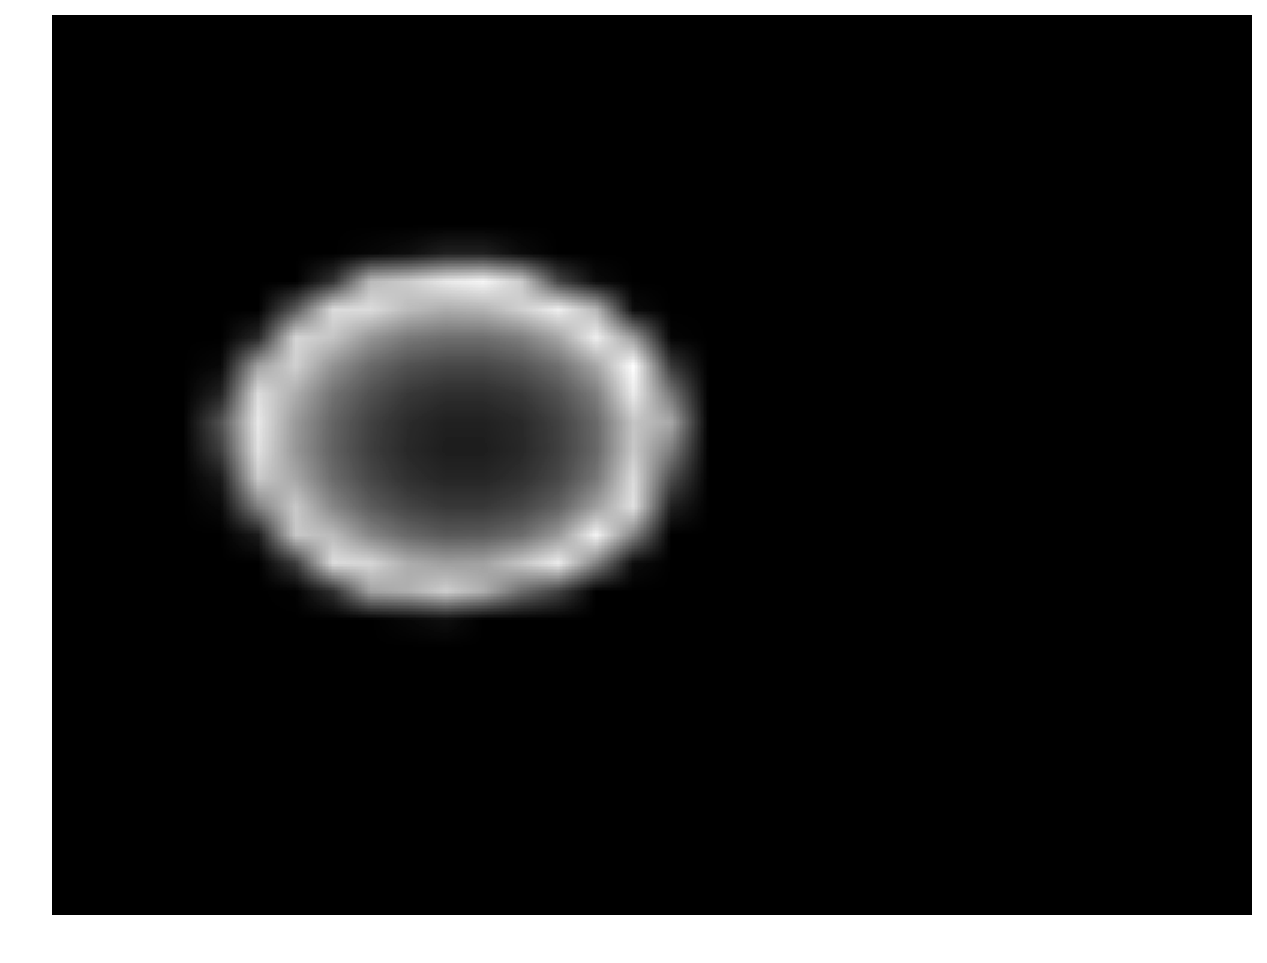
\includegraphics[width=0.75\columnwidth]{figs/depth_example.pdf} \caption{Example Depth Image} \label{fig:depth_image}
        \end{subfigure}
    \begin{subfigure}[t]{0.24\textwidth}
        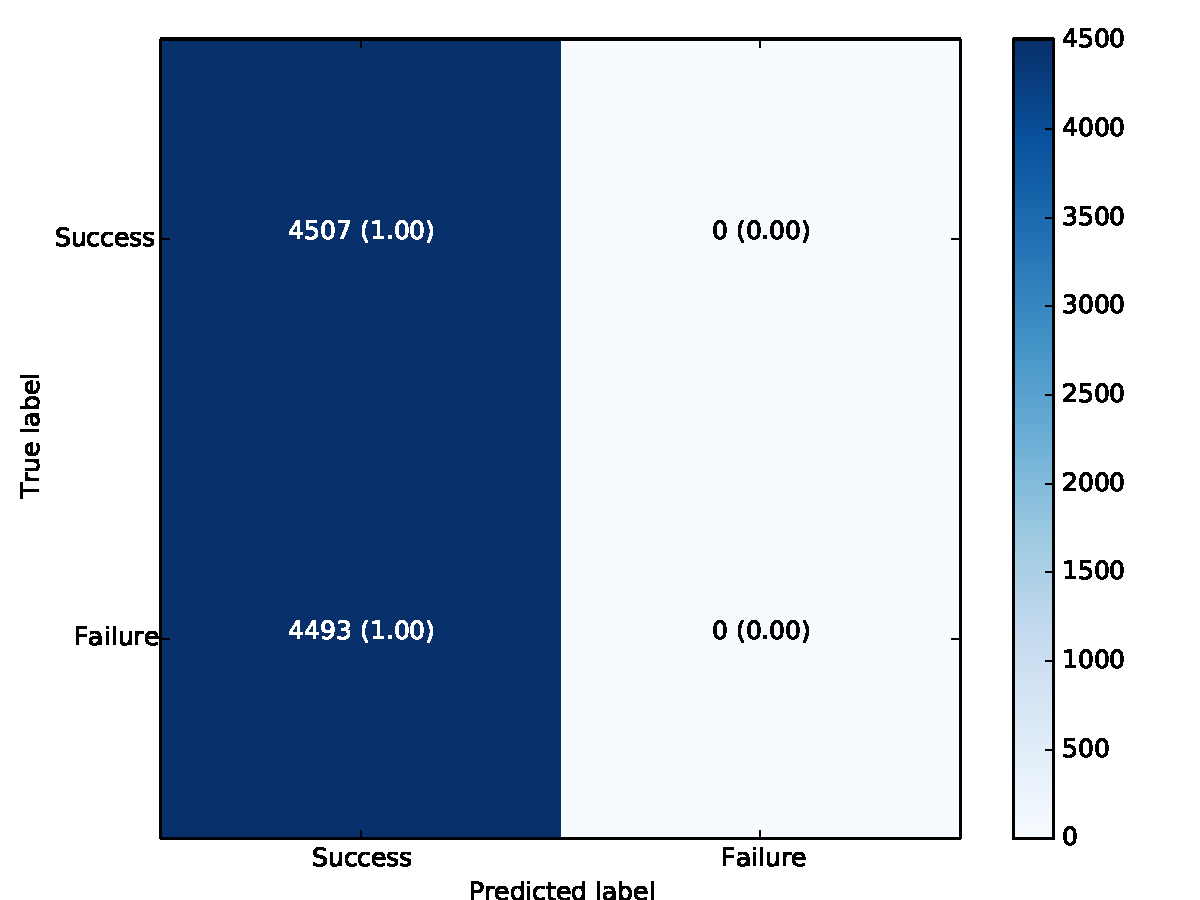
\includegraphics[width=0.9\columnwidth]{figs/balanced_results.pdf} \caption{Balanced Data} \label{fig:balanced_confusion}
    \end{subfigure}
		\begin{subfigure}[t]{0.24\textwidth}
        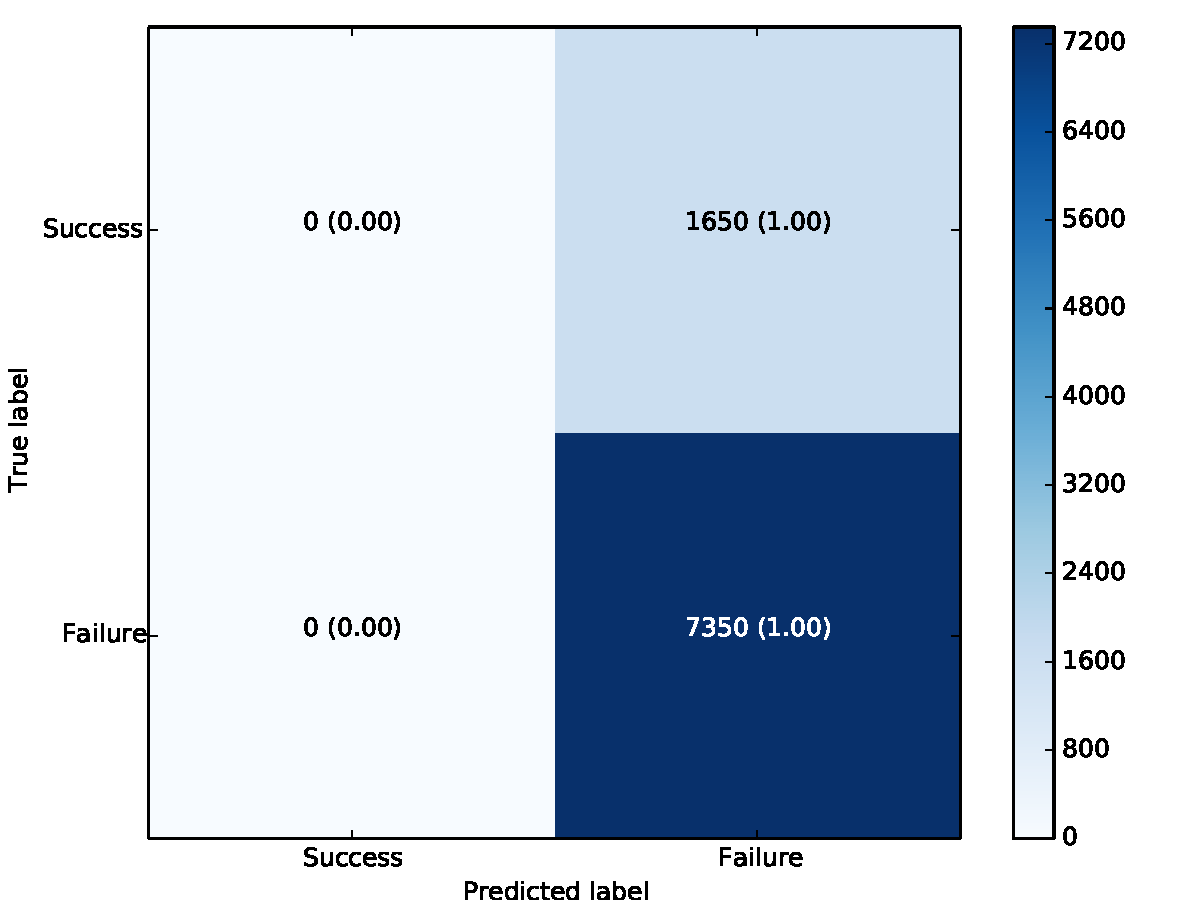
\includegraphics[width=0.9\columnwidth]{figs/unbalanced_results.pdf} \caption{Unbalanced Data} \label{fig:unbalanced_confusion}
        \end{subfigure}
    \begin{subfigure}[t]{0.24\textwidth}
        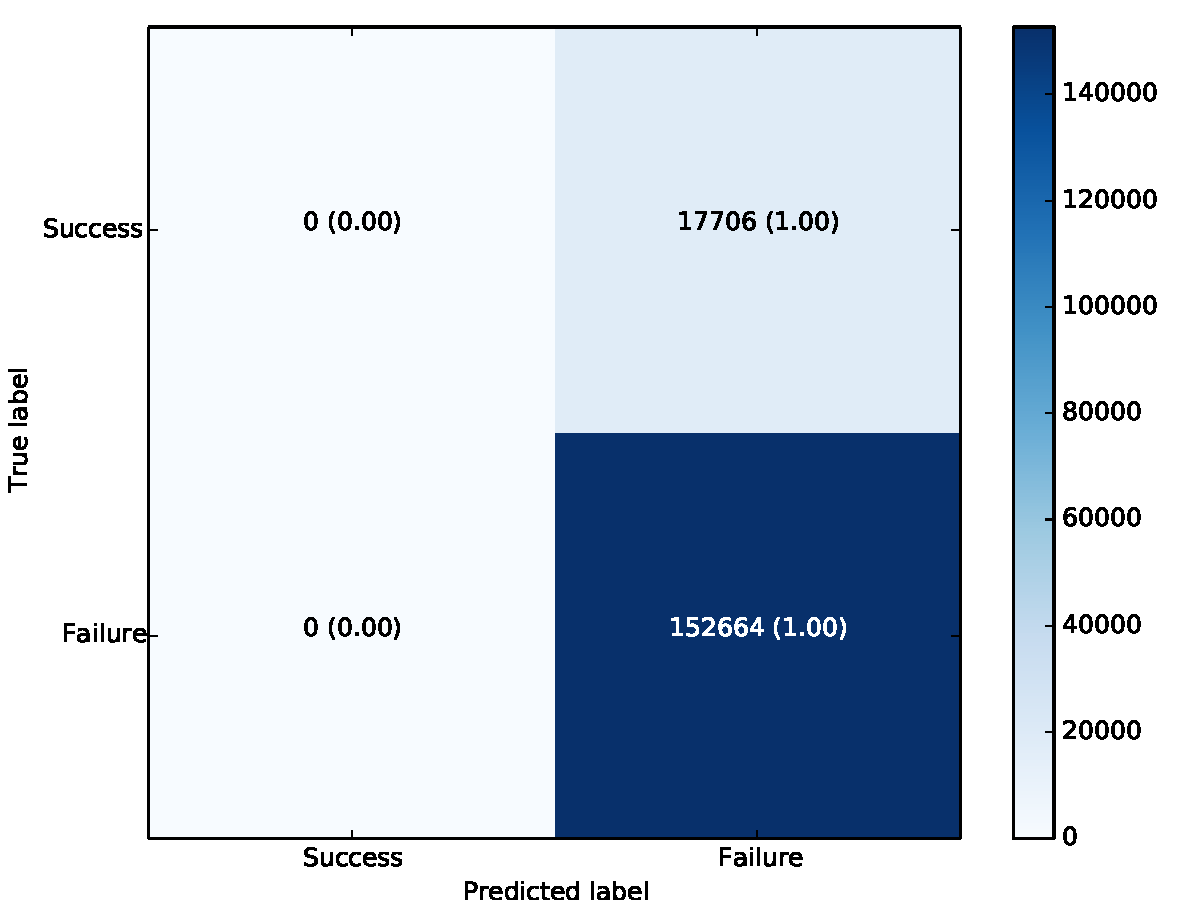
\includegraphics[width=0.9\columnwidth]{figs/paper_original.pdf} \caption{Replicated Paper Results} \label{fig:from_paper}
    \end{subfigure}
\caption{FILL IN CAPTION} \label{fig:confusion_matrices}
\end{figure*}

As mentioned previously, Dex-Net 2.0 contains approximately 20\% positive examples. 
Na{\"i}vely, you could predict a negative label for all instances and be correct 80\% of the time. Interesting, the paper reported an 85.7\% accuracy, which does slightly better than an all negative classifier. 

To investigate this, we begin by using the \rhnote{pretrained dex net network} on the data sets we created by sampling the entire Dex Net data base. 
We can constrain our sampling to produce a data set of 10,000 samples that is 50\% positive examples and 50\% negative examples (referred to as a "balanced" data set). 
Using their network we achieve approximately 50\% accuracy because, as shown in our confusion matrix in \figref{fig:balanced_confusion}, the network learns to always output a positive label. 

If we do not make such a constraint and sample randomly, we expect to have the original distribution: 20\% positive examples and 80\% negative examples (referred to as an "unbalanced" data set). 
As shown by the confusion matrix in \figref{fig:unbalanced_confusion}, the network achieved approximately 80\% accuracy by always guessing negative. 

To confirm our thoughts a step further, we use the data they provide on the network they provide (\rhnote{confirm}). 
This data set is also unbalanced and achieves similarly to above in that it always guesses negative, as seen in \figref{fig:from_paper}. 

This result was initially surprising. 
Due to the few percentage point disparity between our accuracy and theirs, we hesitate to conclusively claim their network did not learn features. 
While we varied the size of the data set we use, we did not come close to their magnitude (in the millions) and therefore it is possible that the network simply needs a tremendous amount of data to learn effectively. 

To explore further, we experiment with varying the architecture of the CNN. 
This both allows us to explore the effect of the architecture (as well as its hyper-parameters) and to see if we can improve upon our accuracy rate. 

\begin{figure*}[t!]
    \centering
    \begin{subfigure}[t]{0.49\textwidth}
        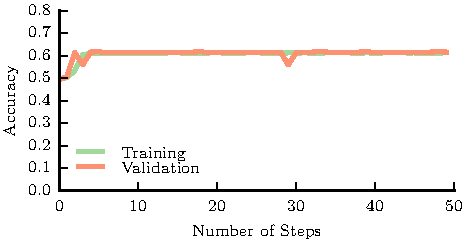
\includegraphics[width=0.9\columnwidth]{figs/gqcnn_accuracy.pdf}
        \caption{Accuracy} \label{fig:accuracy}
        \end{subfigure}
    \begin{subfigure}[t]{0.49\textwidth}
        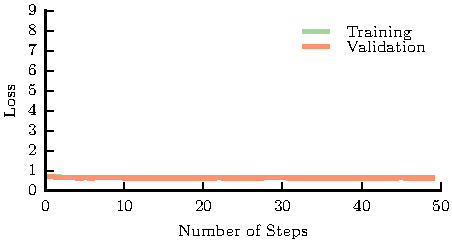
\includegraphics[width=0.9\columnwidth]{figs/gqcnn_loss.pdf}
        \caption{Loss} \label{fig:loss}
    \end{subfigure}
\caption{INSERT CAPTION - gqcnn} \label{fig:gqcnn_results}
\end{figure*}
% !TEX root = main.tex

\section{Testing Architectures}
\label{sec:archs}

We experimented with three types of network architectures, which we call "Inception Net", "Res Net", "Andreas Net". 
Each of these networks are inspired by previous work, but were adapted by us to fit our task. 
For each architecture we will describe their structure, the normalization techniques we applied and the results. 
 
For normalization techniques we applied $L_{1}$ regularization on the fully connected layers, batch normalization on the convolutional layer, and dropout. 
For Inception Net and Res Net, our activation function is the Rectified Linear Unit (ReLu), $f(x) = \max(0, x)$. 
For Andreas Net, our activation function is the Leaky Rectified Linear Unit, $f(x) = \max(a, ax)$ where $a$ is referred to as the slope. 

For each network we plot the accuracy and loss across epochs for the training and validation set and report the final accuracy on the test set. 
We also, for most networks, show the confusion matrix.
For all of the following results we used 50,000 data points (split into 80\%/10\%/10\% for training, validation and testing) from our balanced data set. 

Overall, none of these networks were able to achieve an accuracy rate higher then our re-implemented GQ-CNN. 
We can rank the networks from worst to best by accuracy: Res Net, Inception Net, Andreas Net. 

\subsection{Inception Net}

\begin{figure}[t!]
    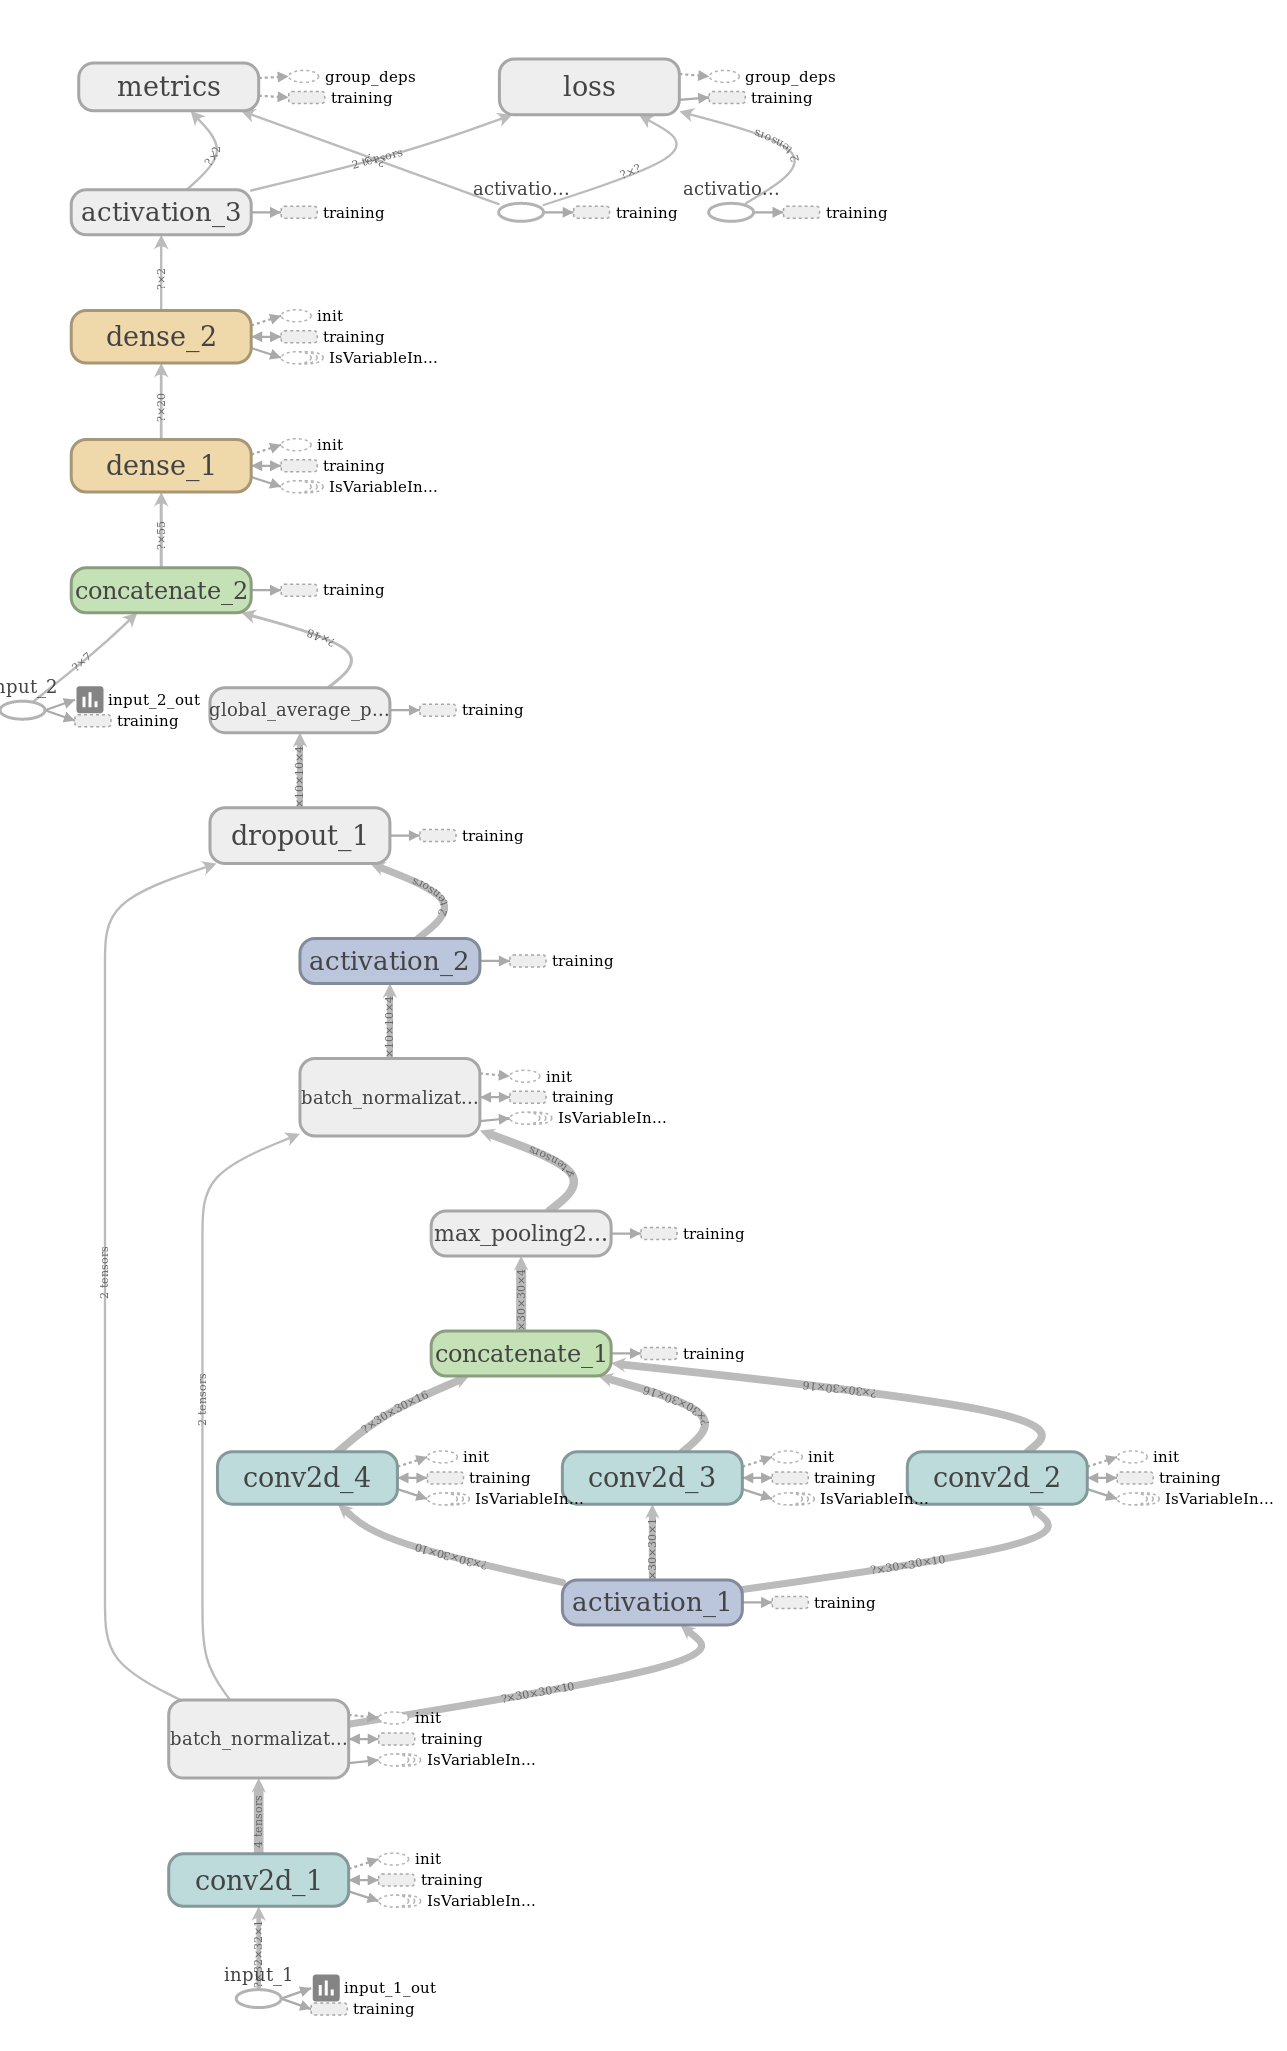
\includegraphics[width=0.99\columnwidth]{figs/inception_net.png}
\caption{Inception Net Architecture. We provide the following labels: Convolution (Conv), Batch Normalization (BN), ReLU (Rectifer Linear Unit), Concatenate (Concat), Dropout (Drop), Global Average Pooling (GAP), Fully Connected (FC), SoftMax (SM).} \label{fig:inception_net}
\end{figure}

The first network architecture we will explore is the Inception Network~\cite{szegedy2015going}, visualized in \figref{fig:inception_net}. 
This network style was originally designed to increase the depth and width of a network while keeping computational load the same while operating on ImageNet~\cite{deng2009imagenet}. 

The inception network begins with 1 convolution layer in the beginning with 10 filters of size 3x3. 
We apply batch normalization to the output of this layer at ReLU as the activation function. 
We then pass that to three parallel convolutional layers of sizes 1x1, 3x3, and 5x5, each with 16 filters. 
These outputs are concatenated on the depth dimension and passed through a max pooling layer of size 3x3 and stride 1x1.
We apply batch normalization, ReLu activation and a dropout of 70\%. 
The outputs are flattened with global average pooling and then the $z$ value is concatenated on. 
We then pass through two fully connected units of size 25 and 2 respectively.  
We apply the softmax function to these final two units to obtain our output for binary classification.

\rhnote{INPUT WHAT WE TRIED}
Our accuracy and loss are shown in \figref{fig:inceptionnet_results}. 
While our training accuracy quickly reaches 70\%, our validation accuracy only rarely spikes above nominal 50\%. 
This poor learning is reflected in the plot of our loss function (\figref{fig:loss_inception}) for our validation set, which never stabilizes. 
Our final accuracy on our training set was 50\%, which, is unimpressive given a binary classification task on a balanced data set. 
Looking at our confusion matrix in \figref{fig:confusion_inception}, our network almost always predicted failure. 
While from a robotic execution perspective this means we are unlikely to execute a failure-likely grasp, the over-prediction of failure also means we are unlikely to execute any grasp. 

\begin{figure*}[t!]
    \centering
    \begin{subfigure}[t]{0.32\textwidth}
        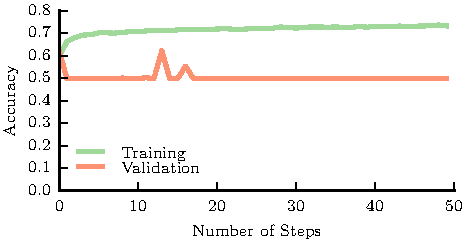
\includegraphics[width=0.9\columnwidth]{figs/inception_accuracy.pdf}
        \caption{Accuracy of Inception Net} \label{fig:accuracy}
        \end{subfigure}
    \begin{subfigure}[t]{0.32\textwidth}
        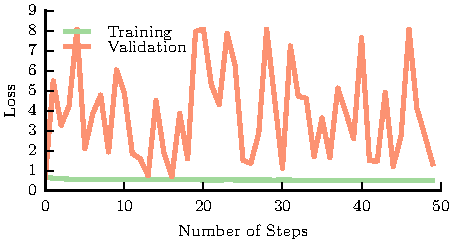
\includegraphics[width=0.9\columnwidth]{figs/inception_loss.pdf}
        \caption{Loss of Inception Net} \label{fig:loss_inception}
    \end{subfigure}
		\begin{subfigure}[t]{0.32\textwidth}
        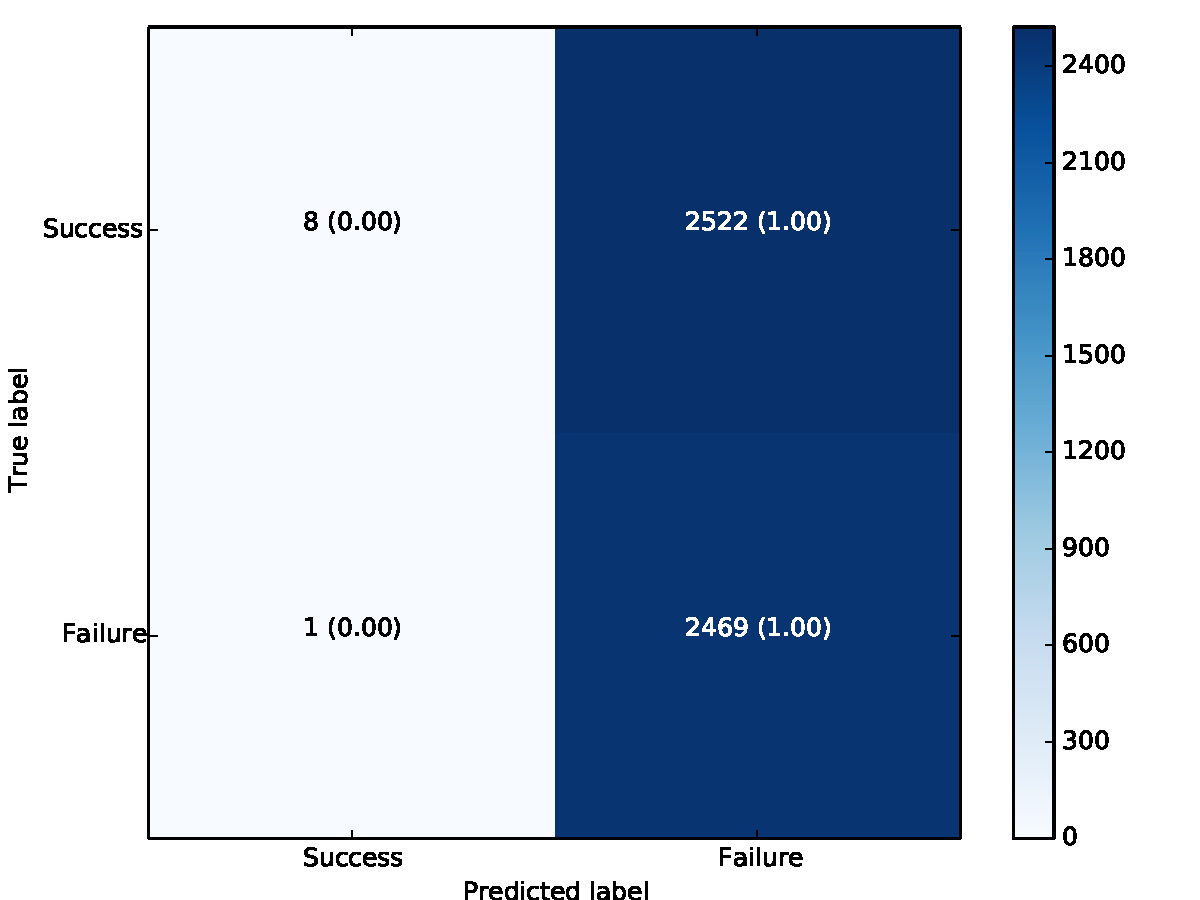
\includegraphics[width=0.8\columnwidth]{figs/confusion_inception.pdf}
        \caption{Confusion Matrix} \label{fig:confusion_inception}
    \end{subfigure}
\caption{We plot the accuracy rate and loss of the Inception Net over training epochs for the training and validation set. This network seems to overfit based off of the difference between the accuracy of the training and validation sets. Our confusion matrix in the rightmost column shows we over predicted failure.} \label{fig:inceptionnet_results}
\end{figure*}


\subsection{Res Net}

\begin{figure}[t!]
    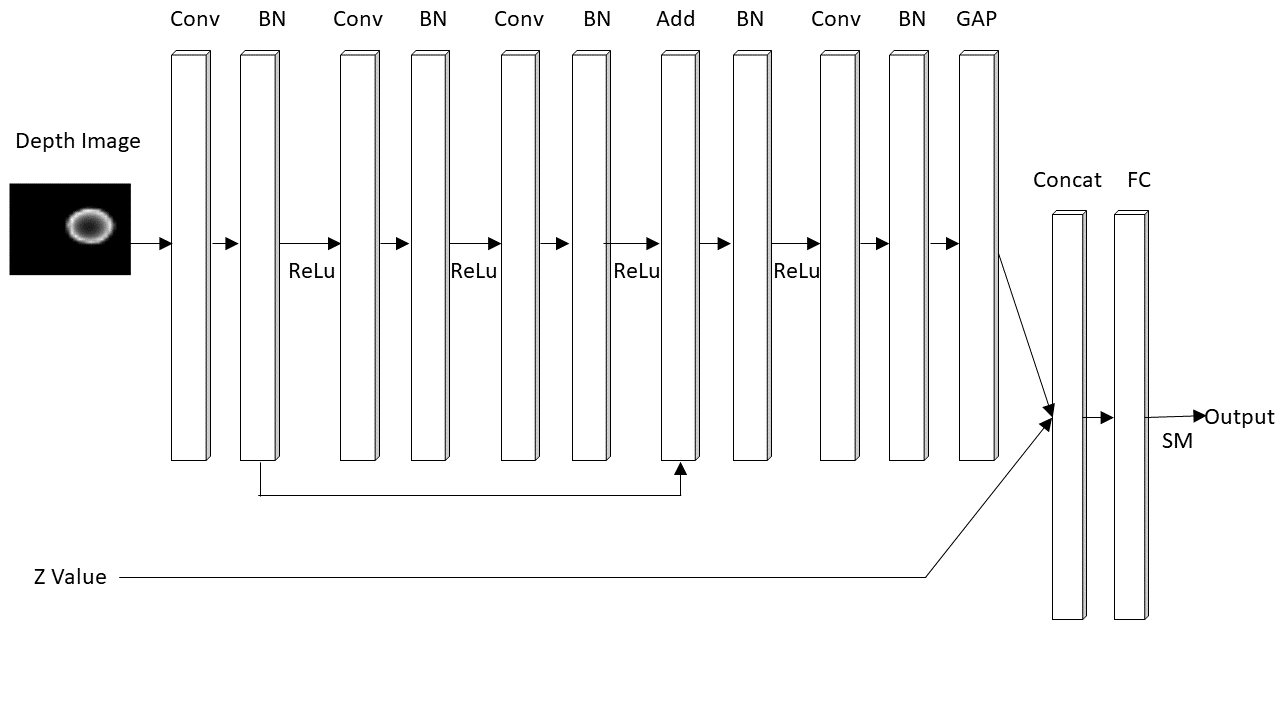
\includegraphics[width=0.99\columnwidth]{figs/res_net.png}
\caption{Res-Net Architecture. We provide the following labels: Convolution (Conv), Batch Normalization (BN), ReLU (Rectifer Linear Unit), Add (Add), Global Average Pooling (GAP), Fully Connected (FC), SoftMax (SM).} \label{fig:res_net}
\end{figure}

Our residual network (called "Res Net" in this discussion) is visualized in \figref{fig:res_net}. 
It consists of one convolutional layer, with 16 filters of size 3x3.
We then apply batch normalization and ReLu as an activation function.
At this point, the output of this layer branches, such that this same output is passed through two more convolution layers of 8 filters 7x7 and 32 filters 3x3used as dimension reduction. 
After each of those two convolution layers is a layer of batch normalization and activation by ReLu.
The output of these two layers is added to their input and then passed through batch normalization and activation by ReLu.
This is then passed to another convolution layer of 8 filters of 1x1 for further dimension reduction. 
We then apply batch normalization and ReLu activation once more before flattened with global average pooling. 

Like for the other network, the $z$ value is concatenated to this output before passing it to a classifier with a fully connected layer of 2 hidden units.
We obtain our output via the softmax function.

\rhnote{insert what we tried}

Our accuracy and loss are shown in \figref{fig:resnet_results}. 
Our training accuracy nears 80\% and our validation accuracy varies between 50\% and 70\%, depending on when we stop our network. 
This stopping criteria is reflected in our loss graph, which also fluctuates for our validation set. 
Doing slightly worse then Inception Net, our final test accuracy is 48\%. 
Looking at our confusion matrix, our learning algorithm over predicted success, in stark contrast to our Inception Net. 
In practice, given the large quantity of false positives, our robot would execute many grasps that are likely to fail, wasting time and resources. 

\begin{figure*}[t!]
    \centering
    \begin{subfigure}[t]{0.32\textwidth}
        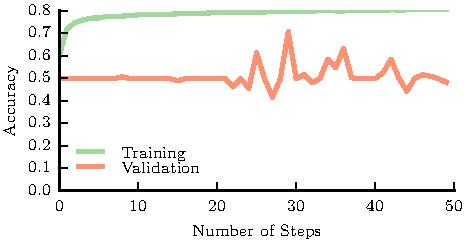
\includegraphics[width=0.9\columnwidth]{figs/res_net_accuracy.pdf}
        \caption{Accuracy} \label{fig:accuracy_res}
        \end{subfigure}
    \begin{subfigure}[t]{0.32\textwidth}
        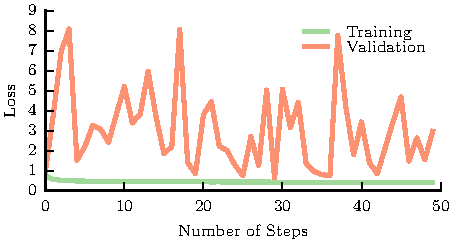
\includegraphics[width=0.9\columnwidth]{figs/res_net_loss.pdf}
        \caption{Loss} \label{fig:loss_res}
    \end{subfigure}
		\begin{subfigure}[t]{0.32\textwidth}
        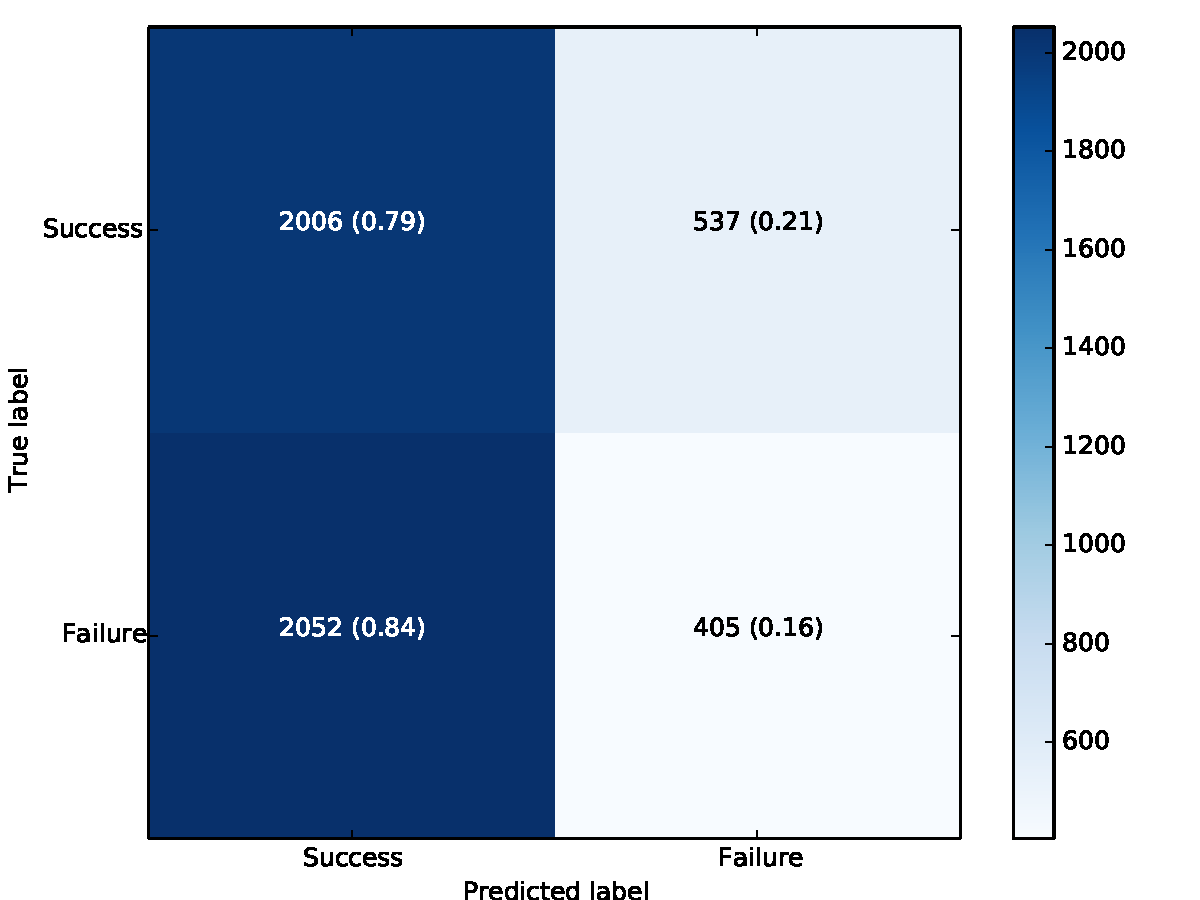
\includegraphics[width=0.8\columnwidth]{figs/confusion_resnet.pdf}
        \caption{Confusion Matrix} \label{fig:confusion_res}
    \end{subfigure}
\caption{We plot the accuracy rate and loss of the Res Net over training epochs for the training and validation set. There is still overfitting in this network, there is odd oscillation of the validation accuracy. Our confusion matrix in the rightmost column shows we over predicted success.} \label{fig:resnet_results}
\end{figure*}

\subsection{Andreas Net}

\begin{figure}[t!]
    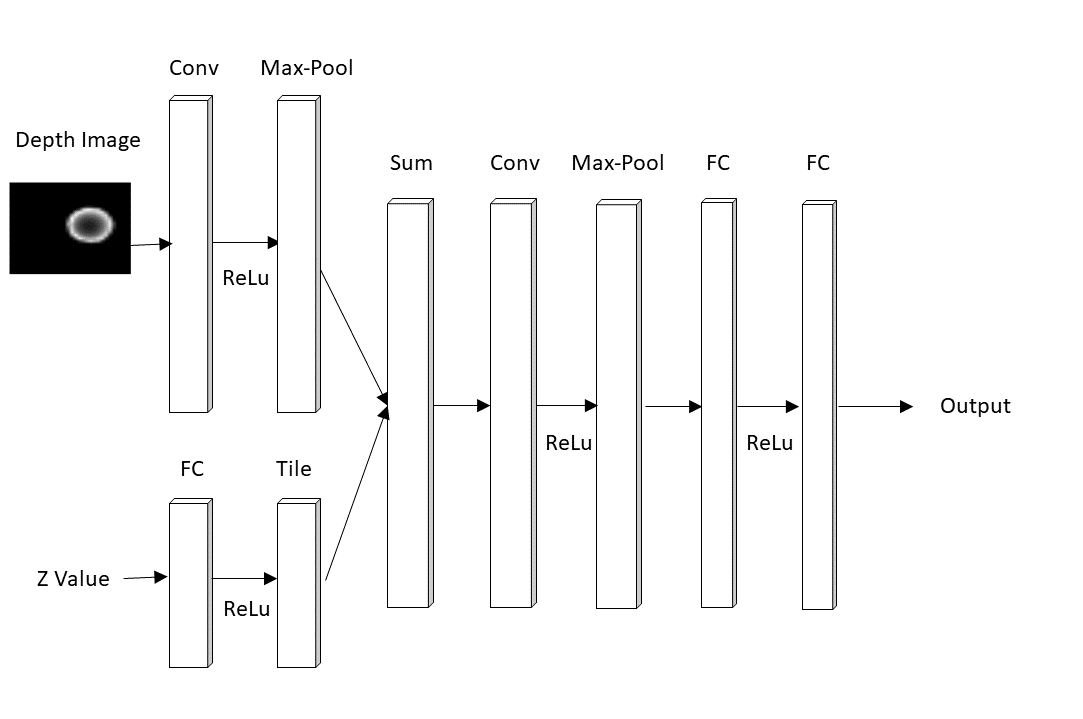
\includegraphics[width=0.99\columnwidth]{figs/andreas_net.png}
\caption{Andreas Net Architecture. We provide the following labels: Convolution (Conv), Leaky Rectified Linear Unit (LR), Max-Pooling (Max-Pool),  Fully Connected (FC), Tiling (Tile), Sum (Sum), Fully Connected (FC), SoftMax (SM).} \label{fig:andreas_net}
\end{figure}

The last architecture we consider is from~\cite{viereck2017learning} and will be referred to as "Andreas Net". 
It is visualized in \figref{fig:andreas_net}. 
The network, like GQ-CNN, was designed for robotics grasping and uses depth images as input. 
However, \cite{viereck2017learning} creates a closed-loop controller that guides the gripper to the object to be grasped. 
Thus their CNN learns the distance to the nearest grasp function used by the controller. 
Despite its original use as a regression network, we adapt it to our classification task. 

The depth image is passed through one convolutional layer, with 20 filters of size 5x5. 
This output is activated by a Leaky ReLu with slope 0.3 before a batch normalization layer. 
We pass this to a max-pooling layer of size 2x2 and stride 1x1. 
The z-value is passed through a full connected layer of 20 units with $L_{1}$ regularization of $\lambda=0.1$.
We pass this through Leaky ReLu, again with slope 0.3, and then tile the output~\cite{ngiam2010tiled}.
The outputs of each of these, the processed depth image and processed z-value, are summed.

This result is passed through convolutional layer with 50 filter of size 5x5, followed by Leaky ReLu, with slope 0.3. 
We then apply dropout at rate 0.6 and then a max-pooling layer with size 2x2 and stride 1x1. 
We flatten this output and pass it through a fully connected layer of 20 units and $L_{1}$ regularization with $\lambda = 0.1$. 
This is activated by Leaky ReLU (again slope 0.3) and finally connected to a fully connected layer with 2 hidden units (again with $L_{1}$ regularization at $\lambda=0.1$). 
We apply softmax to these two units to generate our output. 

\rhnote{what we tried}

Our accuracy and loss are shown in \figref{fig:andreas_results}. 
After 30 training steps, our training and validation accuracy improve with our training accuracy near 70\% and our validation wavering between 50\% and 70\%, depending on when we stop training. 
For both networks our loss over time shows little variance. 
Our final test accuracy is 56\%, an improvement over Inception Net and Res Net, but still slightly worse then our re-trained version of the GQ-CNN. 

\begin{figure*}[t!]
    \centering
    \begin{subfigure}[t]{0.49\textwidth}
        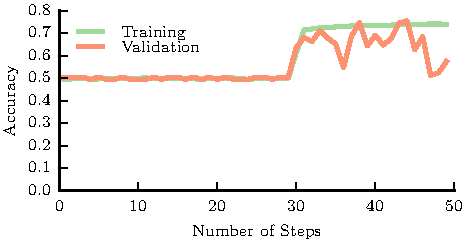
\includegraphics[width=0.9\columnwidth]{figs/andreas_accuracy.pdf}
        \caption{Accuracy} \label{fig:accuracy}
        \end{subfigure}
    \begin{subfigure}[t]{0.49\textwidth}
        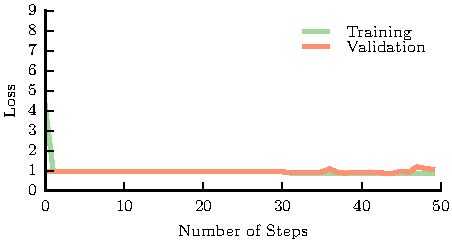
\includegraphics[width=0.9\columnwidth]{figs/andreas_loss.pdf}
        \caption{Loss} \label{fig:loss}
    \end{subfigure}
\caption{We plot the accuracy rate and loss of the Andreas Net over training epochs for the training and validation set. Of our new networks this performs the best, although its validation accuracy also oscillates.} \label{fig:andreas_results}
\end{figure*}
% !TEX root = main.tex

\section{Discussion}
\label{sec:discussion}
\rhnote{mention gqcnn generalized better}

The goal of this project was to use modified depth images to perform binary classification whether a grasp would succeed, as measured by a grasp stability metric. 
We leveraged the recently published Dex Net 2.0 data base by sampling data points~\cite{mahler2017dex}. 

We began by learning using the Dex Net framework, their GQ-CNN, with various input sampling techniques. 
Aiming for better performance we next experimented with three architectures: Inception Net, Res Net and Andreas Net. 

Overall, we did not achieve the accuracy we were hoping for. 
Taking a step back, we hypothesize three possible reasons. 
The first is that, although we tried various networks, we did not find the best possible network or combination of hyperparameters. 
To investigate this, we would continue experimenting with architectures. 

Our second guess is that we did not train our network with enough data. 
For computational reasons, we sampled sets from the large Dex Net database and thus trained on a much smaller set. 
The key to this kind of learning is large quantities of data, so is possible our issues would be alleviated by training on larger sets. 
While we were able to achieve comparable performance (on a re-scaled data set), the GQ-CNN is reported to have 4.5 million trainable parameters, which means that we had many more parameters then data points. 

Our third possible reason relates to the nature of the data set. 
Considering we did not create the data set, editing it in a significant way was outside of our control. 
It is possible that the depth image and distance is not sufficiently powerful enough representation to learn grasp stability. 
Several other grasp learning algorithms leverage a color input, since color can often characterize objects~\cite{zeng2017robotic}.  
While we attempted to access a data set with color images, the repository was not usable in its published form (it referenced data that was not publicly accessible) and the authors of the repository did not reply to our several inquires. 

Our learning objective is a hotly published research area and much of the work we reference is extremely recent (i.e. Dex Net 2.0 was presented in July of this year and Andreas Net was published to Arvix less than a month ago). \rhnote{some conclusion sentence!}

%\addtolength{\textheight}{-12cm}

\section*{ACKNOWLEDGMENT}
We would like to thank the entire course staff for making this course possible and our project TA for his helpful guidance. 
We would also like to thank Jeff Mahler and Sherdil Niyaz (a few of the authors of the DexNet 2.0 paper) for answer our questions throughout this project. 

\section*{Division of Labor and Code}
Both partners contributed evenly throughout the duration of the project. 
We collaborated in design our research questions, areas of exploration and design. Rachel took the lead on processing the data set, figure generation and writing the final results. Sebastiani took the lead on designing the network hyper-parameters and training the networks. 
Our code base is available at: \url{https://github.com/finalProject6867}

{\footnotesize
    \bibliographystyle{ieeetr}
\bibliography{../references}}

\end{document}
